%!TEX root = ../../Main.tex

\subsection{Задача 1}

Розглянемо задачу:
%%%
\begin{equation}\label{eq:problem1}
\begin{cases}
	- \Delta u(x_1,x_2) + 1000u(x_1, x_2) = f(x_1,x_2), \\
	f(x_1,x_2) = (18 \pi^2 +1000)\sin(3 \pi x_1) \sin (3 \pi x_2), \\
	u|_\Gamma = 0 ,\\
	\Omega = \left[0;1\right] \times \left[0;1\right].
\end{cases}
\end{equation}
%%%
Її точний розв'язок
%%
\begin{equation}
	u(x_1,x_2) = \sin(3 \pi x_1) \sin (3 \pi x_2)
\end{equation}
%%
зображений на \autoref{plot:problem1_exact}.
%%
\begin{figure}[H]
	\centering
    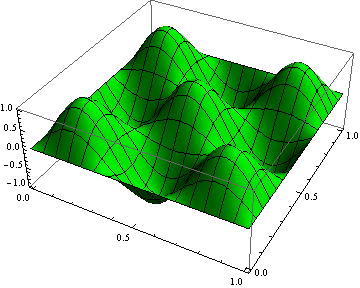
\includegraphics[scale=1.0]{problem1/ExactSolution}
    \caption{Точний розв'язок задачі \eqref{eq:problem1}. $u(x_1,x_2) = \sin(3 \pi x_1) \sin (3 \pi x_2)$}
    \label{plot:problem1_exact}
\end{figure}
%%%
Задамо граничну точність апроксимації на скінченному елементі в 5\%.
За початкове розбиття виберемо рівномірне на сітці 10x10 (\autoref{fig:init_mesh1}).
%%
\begin{figure}[H]
	\centering
    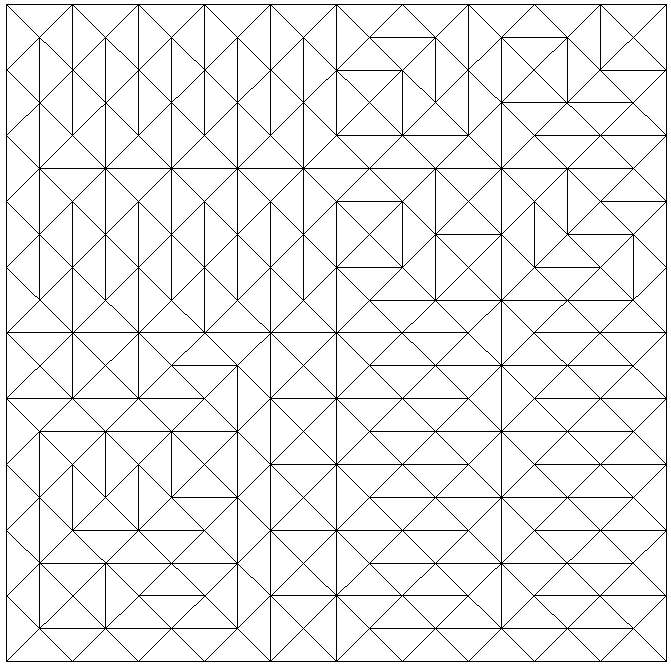
\includegraphics[scale=0.7]{problem1/InitialMesh}
    \caption{Початкове розбиття на скінченні елементи.}
    \label{fig:init_mesh1}
\end{figure}


Для отримання похибки в 5\% знадобилося 18 кроків та \nn{19322} скінченних елементи. Графіки апроксимацій на різних кроках обчислення зображені на \autoref{fig:p1_solution1}-\ref{fig:p1_solution18}:
%
\begin{figure}[H]
	\centering
    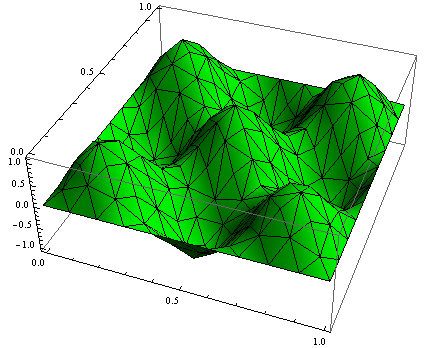
\includegraphics[scale=0.9]{problem1/my/solutions/1}
    \caption{$u_h(x)$ на першому кроці. Кількість скінченних елементів - \nn{400}.}
    \label{fig:p1_solution1}
\end{figure}
%
\begin{figure}[H]
	\centering
    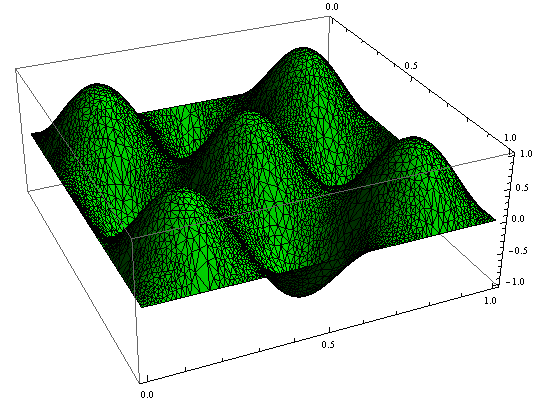
\includegraphics[scale=0.7]{problem1/my/solutions/5}
    \caption{$u_h(x)$ на 5-му кроці. Кількість скінченних елементів - \nn{12903}.}
    \label{fig:p1_solution5}
\end{figure}
%
\begin{figure}[H]
	\centering
    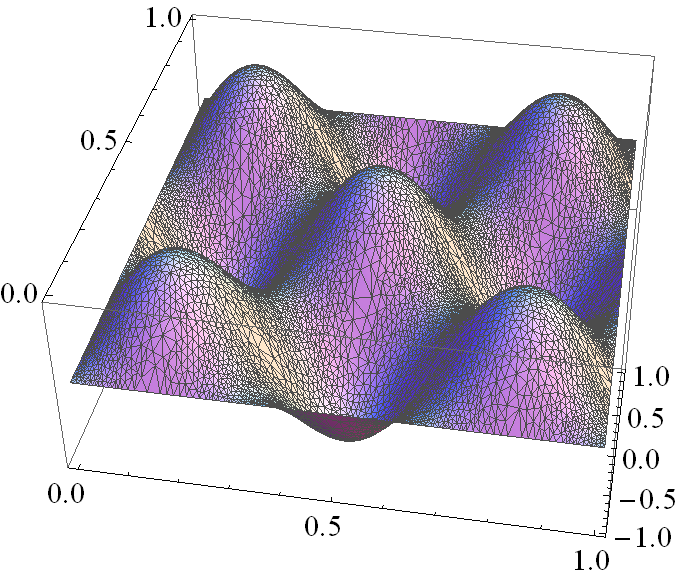
\includegraphics[scale=0.7]{problem1/my/solutions/18}
    \caption{$u_h(x)$ на 18-му кроці. Кількість скінченних елементів - \nn{19322}.}
    \label{fig:p1_solution18}
\end{figure}
%
\clearpage
Графіки індикаторів похибок на скінченних елементах зображено на \autoref{fig:p1_aee1} - \autoref{fig:p1_aee18}.
%
\begin{figure}[H]
	\centering
    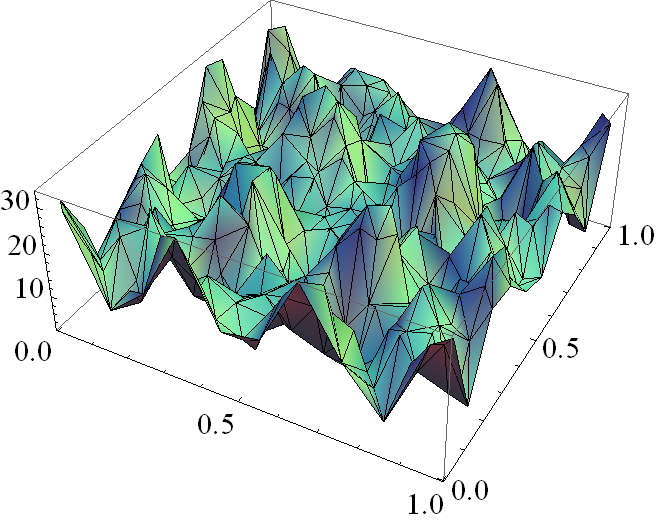
\includegraphics[scale=0.8]{problem1/my/AEE/1}
    \caption{Індикатори похибки на першому кроці. Кількість скінченних елементів - \nn{400}.}
    \label{fig:p1_aee1}
\end{figure}

\begin{figure}[H]
	\centering
    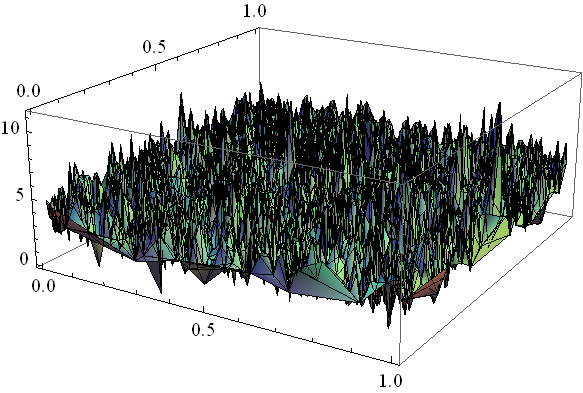
\includegraphics[scale=0.85]{problem1/my/AEE/5}
    \caption{Індикатори похибки на 5-му кроці. Кількість скінченних елементів - \nn{12903}.}
    \label{fig:p1_aee5}
\end{figure}

\begin{figure}[H]
	\centering
    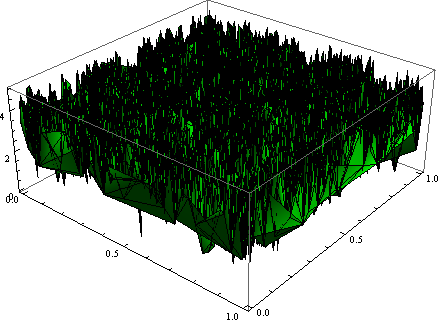
\includegraphics[scale=0.85]{problem1/my/AEE/18}
    \caption{Індикатори похибки на 18-му кроці. Кількість скінченних елементів - \nn{19322}.}
    \label{fig:p1_aee18}
\end{figure}

З \autoref{fig:p1_aee18} бачимо, що отримане розбиття характеризується тим, що похибка розділена майже рівномірно по всіх скінченних елементах.

Нижче в таблиці наведено деякі показники отриманих розбиття та наближень на кроках адапативної схеми.
%
\pgfplotstabletypeset[col sep=comma,
	columns={0,1,2,4,5,6,7,3},
	columns/0/.style={
		column name=\textnumero
	},
	columns/1/.style={
		column name=$N(h)$
	},
	columns/2/.style={
		column name=$M(h)$
	},
	columns/3/.style={
		column name=$\norm{e_h}^\prime$
	},
	columns/4/.style={
		column name=$\norm{e_h}$
	},
	columns/5/.style={
		column name=$\norm{e}$
	},
	columns/6/.style={
		column name=${P[H_1, u_h]}$
	},
	columns/7/.style={
		column name=$\frac{\norm{e_h}}{\norm{e_h+u_h}}*100\%$
	},
%%
	begin table=\begin{longtable},
	end table=\end{longtable},
%
	every head row/.style={before row=\caption{Похибки та збіжність схеми.}\\\toprule, after row=\midrule},
	every last row/.style={after row=\bottomrule},
	every nth row={1}{before row=\midrule},
	column type/.add={|}{|}
]{include/8NumResults/problem1/my/errors/table.csv}
%
Тут:
\begin{equation*}
	\begin{split}
		&\norm{e_h^\prime} \text{ - оцінювач похибки представлений в \cite{OstShynAee11}, } \\
		&\norm{e_h} \text{ - оцінювач похибки представлений в даній роботі,} \\
		&\norm{e} \text{ - реальна похибка,} \\
		&P[H_1, u_h]_i = 2*\frac{\ln{\norm{e_h^{i-1}}}-\ln{\norm{e_h^i}}}{\ln{N_i}-\ln{N_{i-1}}} \text{ - показник збіжності.} \\
	\end{split}
\end{equation*}
%
Всі норми обраховано в $H_1(\Omega)$. Наведемо також графік збіжності норм похибок.
%
\begin{figure}[H]
	\centering
    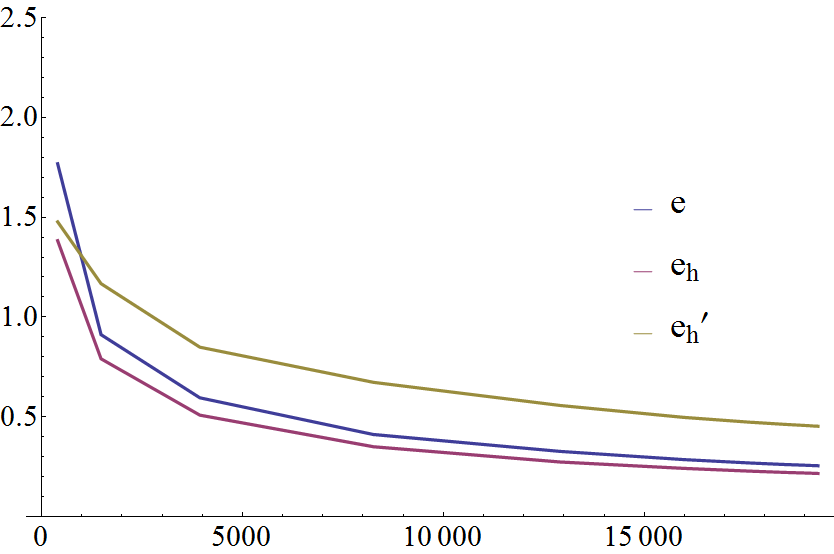
\includegraphics[width=\textwidth]{problem1/my/Plotnb}
    \caption{Збіжність норм похибок МСЕ із збільшенням кількості елементів.}
    \label{fig:p1_my_errors}
\end{figure}

Якщо ж за основу для адаптивної стратегії взяти оцінювач з \cite{OstShynAee11}, то таблиця обчислених результатів матиме вигляд:
%
\clearpage
\pgfplotstabletypeset[col sep=comma,
	columns={0,1,2,3,5,6,7,4},
	columns/0/.style={
		column name=\textnumero
	},
	columns/1/.style={
		column name=$N(h)$
	},
	columns/2/.style={
		column name=$M(h)$
	},
	columns/3/.style={
		column name=$\norm{e_h^\prime}$
	},
	columns/4/.style={
		column name=$\norm{e_h}$
	},
	columns/5/.style={
		column name=$\norm{e}$
	},
	columns/6/.style={
		column name=${P[H_1, u_h]}$
	},
	columns/7/.style={
		column name=$\frac{\norm{e_h^\prime}}{\norm{e_h^\prime+u_h}}*100\%$
	},
%%
	begin table=\begin{longtable},
	end table=\end{longtable},
%
	every head row/.style={before row=\caption{Похибки та збіжність схеми.}\\\toprule, after row=\midrule},
	every last row/.style={after row=\bottomrule},
	every nth row={1}{before row=\midrule},
	column type/.add={|}{|}
]{include/8NumResults/problem1/ost/errors/table.csv}

\clearpage
Графік залежності похибки від кількості елементів має вигляд:

\begin{figure}[H]
	\centering
    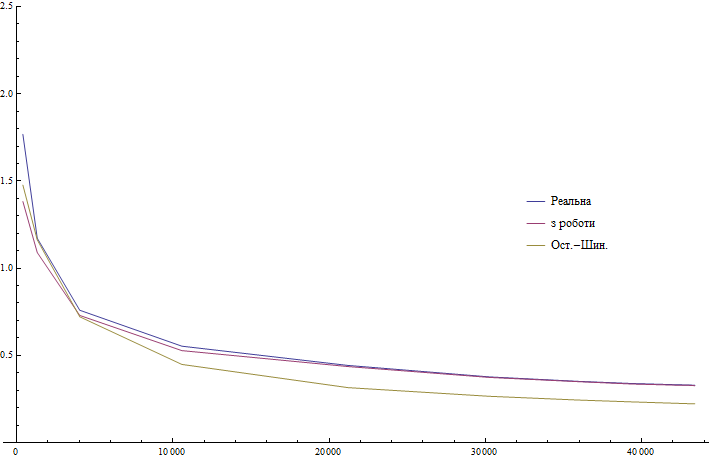
\includegraphics[width=\textwidth]{problem1/ost/Plotnb}
    \caption{Збіжність норм похибок із збільшенням кількості елементів.}
    \label{fig:p1_ost_errors}
\end{figure}

Як бачимо на розглянутій задачі оцінювач, запропонований в роботі, досягає кращої точності (норма похибки 0.25 проти 0.33), використовуючи вдвічі меншу кількість елементів (\nn{19322} проти \nn{43399}) порівняно із оцінювачем з \cite{OstShynAee11}.

На більшій кількості елементів якість отриманої оцінки вища, ніж оцінки отриманої в \cite{OstShynAee11},
навіть якщо за основу для адаптації вибрано оцінювач $e_h^\prime$, що добре видно на \autoref{fig:p1_ost_errors}.
